% Meta-info: Java version, build environment, RMI
\subsection{Environment}
\paragraph{}{
    To build the Gcom project, you need a working distribution of maven, java
 1.7 or above. Some scripts are available in the \texttt{bin}, assuming
 you use bash.
}


% Building JAR
\subsection{Compiling Gcom}
\paragraph{}{
    To use the Gcom artifact, you need to compile and package it. To do so,
 just run \texttt{\$ mvn package} in the Gcom folder. The sub-directory
 \texttt{target} may now contain two jar files, \texttt{Gcom-4.2.jar} and
 \texttt{Gcom-4.2-jar-with-dependencies.jar}. The first one can be imported
 to a new project and can be used as a library. The second jar file is the 
 project packed with all needed dependencies and can be use to run directly
 the name server needed by Gcom.
}

% Starting nameserver
\subsection{Name Server}
\paragraph{}{
    To r
}

% Demo chat-app description
\subsection{Gchat, the toy demo of Gcom}
\paragraph{}{
    To show off and prove Gcom works, we build a demonstration application,
 Gchat. It is basically a chat build on top of Gcom.
}

\begin{figure}[h]
    \begin{center}
        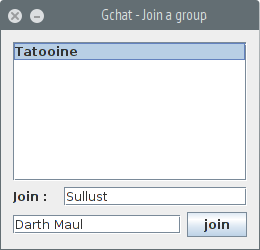
\includegraphics[scale=0.6]{figures/gchat_connection.png}
    \end{center}
    \caption{Connection window of gchat}
    \label{fig:gchat_connect}
\end{figure}

\paragraph{}{
    The application can be found in the sub-directory \texttt{Gchat}. 
 A script in the \texttt{bin} directory allow you to run the application easily
 by running \texttt{ \$ ./chat.sh}. If need, the application can be (re)compiled by
 giving \texttt{compile} as an argument of the application. Finally you can run
 the debug mode by adding \texttt{debug} to the arguments.
}

\begin{figure}[h]
    \begin{center}
        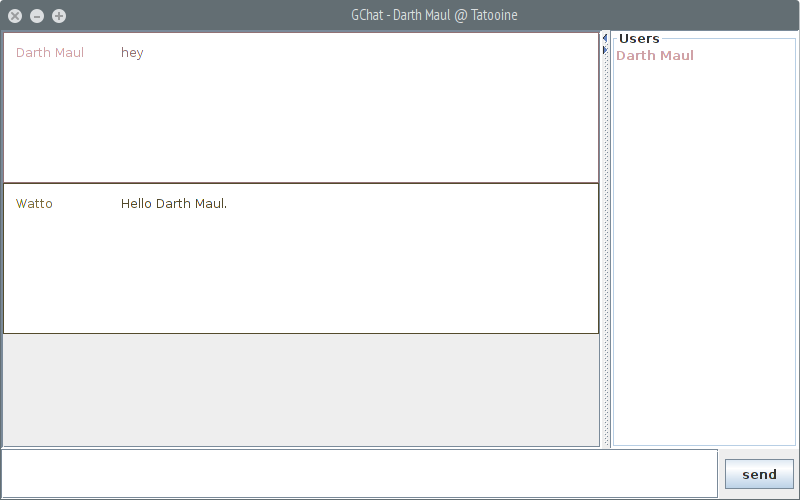
\includegraphics[scale=0.4]{figures/gchat_chat.png}
    \end{center}
    \caption{Chat window of gchat}
    \label{fig:gchat_connectchat}
\end{figure}

% Starting client and creating or joining group
\paragraph{}{
    The application uses two windows. The first one is the connection window, where
 the user can chose a name and the group to join. The second window if the main
 window used to chat with the users that join the same group.
}


% Further dev 
	% Create own application using Gcom
	
\begin{figure}[h]
    \begin{center}
        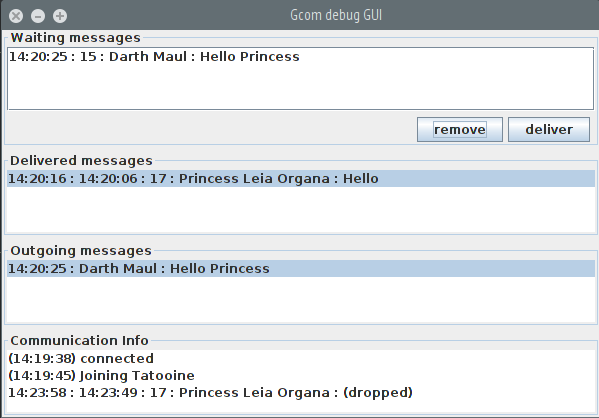
\includegraphics[scale=0.5]{figures/debug_window.png}
    \end{center}
    \caption{Debug interface of Gcom}
    \label{fig:debugGui}
\end{figure}

% trouble shooting ?
\subsection{Trouble shooting}
\paragraph{}{
    The main problem you can get may concern the name server.
}

